\chapter{Consistent Algorithms}
Our goal in this chapter will be to simultaneously achieve sublinear regret and minimize some notion of {\em consistency} cost. We first \dots (\textbf{TODO: complete the exposition here.})

\section{Consistency Cost}
A possible notion for consistency cost is the number of times the player changes her decision in $T$ rounds, \ie,
\begin{equation}\label{eq:consistencycostdef}
    \kappa_T := \sum_{t = 2}^T \mathbf{1}_{x_{t} \not= x_{t - 1}}.
\end{equation}
We note that there are different possible notions of consistency, all dependent on the respective application. As an example, in the situation of online discrete submodular maximisation, where at each round the player plays a \emph{subset} $S_t \subseteq V$ and the loss functions are submodular, a notion of consistency cost can be defined as 
\begin{equation}\label{eq:consistencycostset}
    \kappa'_T := \sum_{t=2}^T |S_t \triangle S_{t-1}|,
\end{equation}
where $A\triangle B$ is the symmetric difference of $A$ and $B$. In other situations where the decision space is a general metric space $(\Xcal, d)$, one can define the consistency cost to be
\begin{equation}\label{eq:consistencycostmetric}
    \kappa''_T := \sum_{t=2}^T d(x_t, x_{t-1}).
\end{equation}
As an example, the cost \eqref{eq:consistencycostdef} becomes a special case of \eqref{eq:consistencycostmetric}, when one puts the \emph{discrete metric} on $\Xcal$. Moreover, \eqref{eq:consistencycostset} is a special case, when one take $d(A, B) = |A\triangle B|$ to be a metric on the discrete hypercube.

Keeping each of these costs small\footnote{with a correct interpretation of smallness.} will result in different behaviours of the online algorithm. The first cost encourages the algorithm to \emph{stick} to the previously played decisions. The second cost makes the algorithm to change the elements of the selected set as little as possible; it keeps a bag of items and change the items in the bag as few times as possible. The third one trys to \emph{move} as little as possible in the decision space.

In what follows, we take \eqref{eq:consistencycostdef} as the defintion of cosistency cost.

\section{Decision Paths}
Under the assumption of Lipschitz loss functions, upper bounds on regret can be obtained by bounding the amount one \emph{moves} in the decision space. This brings us to the notion of a \emph{decision path}.

\begin{definition}[Decision Path]
    For a sequence of points $(x_t)_{t\in[T]} \subset \RR^d$ we define the decision path to be the sequence of non-negative real numbers $(p_t)_{t\in [T]}$ such that $p_1= 0$ and for all $t > 1$,
\[
  p_t - p_{t-1} = \|x_t - x_{t-1}\|.
\]
\end{definition}
Intuitively, if we had to move a pebble from $x_{t-1}$ to $x_t$ as the algorithm went on, $p_t$ would represent the total distance traveled by the pebble after $t$ steps, see Figure~\ref{fig:decisionpath} for an illustration.
\begin{figure}[h!]
    \centering
    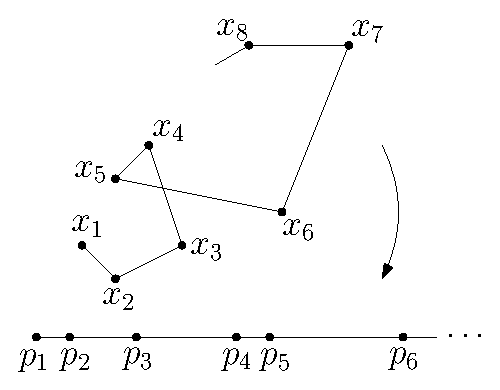
\includegraphics[width=5cm]{figures/decision-path}
    \caption{The Decision Path}
    \label{fig:decisionpath}
\end{figure}

For analytic reasons that become apparent in later sections, we also introduce the \emph{$\delta$-padded decision path} as follows. 
\begin{definition}[$\delta$-padded Decision Path]
Let $\delta = (\delta_t)_{t\in\NN}$ be an increasing sequence of positive numbers and  $p_1, \ldots, p_T$ be a decision path. Then the corresponding $\delta$-padded decision path is the sequence $r_1, \ldots, r_T$ with $r_1 = p_1$ and $r_t = p_t + \delta_t$ for $t>1$.
\end{definition} 

Any online algorithm whose decision space is a subset of Euclidean space, naturally defines a decision path: take $x_t$ to be the decision made at round $t$. For the special case of the OGD algorithm, one has the following lemma for the length of the corresponding decision path. 
\begin{lemma}
  Let $f_t\in C^1_L(\Xcal)$ be convex for all $t\in[T]$ and $(x_t)$ be the sequence of decisions made by OGD. Assume that $(p_t)$ is the decision path for $(x_t)$.
  \begin{enumerate}[label=(\roman*)]
      \item Using step size $\eta_t = \frac{D}{L}t^{-1/2}$, one has for all $t \in [T]$,
         \[ p_t \leq  2D \sqrt{t}. \]
     \item If in addition, $f_t$ are $\alpha$-strongly convex for all $t\in [T]$, then using step size $\eta_t=\frac{1}{\alpha t}$,
         \[ p_t \leq \tfrac{L}{\alpha}(1+\log t). \]
  \end{enumerate}
  \label{lem:ogdpathlength}
\end{lemma}
\begin{proof}
    By the OGD update rule, the Projection Lemma \ref{lem:projection}, and Lipschitz continuity of $f_t$, one gets
 \begin{align*}
   p_{t+1}-p_t &= \|x_{t+1} - x_t\| \\
   &= \|\mathrm{Proj}_\Xcal(x_t - \eta_t\nabla f_t(x_t))-x_t\| \\
  &\leq \|x_t - \eta_t\nabla f_t(x_t)-x_t\| \\
  &= \eta_t\|\nabla f_t(x_t)\| \leq \eta_t L.
 \end{align*}
Since $p_1 = 0$ one can write
\[
  p_t = \sum_{j=1}^{t-1} (p_{j+1} - p_j) \leq L\sum_{j=1}^{t-1} \eta_j.
\]
For (i), we have $\eta_t = \frac{D}{L\sqrt{t}}$ and
   \[
   p_t \leq L\sum_{j=1}^{t-1} \frac{D}{L\sqrt{j}} \leq D \int_0^{t-1} z^{-\frac{1}{2}}\,dz \leq 2D\sqrt{t}.
 \]
% meaning that $r_n \leq (2D + \delta)\sqrt{n}$.
For (ii), we have $\eta_t = \frac{1}{\alpha t}$ and
  \[
    p_t \leq L \sum_{j=1}^{t-1} \frac{1}{\alpha j} \leq \frac{L}{\alpha}(1+\log t).
 \]
\end{proof}

\section{Towards No-Regret Consistent Algorithms}

In order to achieve a trade-off between regret and consistency, our algorithm will make use of a basic algorithm $\Acal$, such as OGD, and decide probabilistically at each time step whether to update the current solution point to $\Acal$'s proposal, or to stick to the one from the previous round. Intuitively, we want the updates to be more likely to happen if the current solution point is far away from the $\Acal$'s newly proposed point, but also less likely to happen as the algorithm proceeds and starts converging to a near-optimal solution. As in a Poisson process, the distribution of inter-arrival times is dependent on the \emph{length} of the interval, we will update the algorithm's solution whenever a specific point process on the padded decision path has a hit. 

Concretely, let $\lambda: \RR_+ \to \RR_+$ be an increasing intensity function we will define later. Also define $(r_t)_{t\leq T}$ to be the padded decision path of $\Acal$. We will update the strategy at time $t$ if and only if the non-homogeneous Poisson process with rate $\lambda(\tau)$ had a non-zero count in the interval $(r_{t-1}, r_t].$ This is equivalent to updating with probability  $1 - \exp(-\int_{r_{t-1}}^{r_t} \lambda(\tau)\, d\tau)  = 1 - \exp\{-(M(r_t)- M(r_{t-1}))\}$. Figure~\ref{fig:poisson} shows an example of the Poisson process and updating procedure.

\begin{figure}[h!]
    \centering
    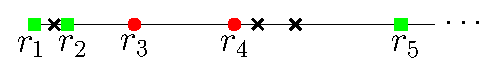
\includegraphics[width=5cm]{figures/poisson}
    \caption{Let $(r_t)$ be the padded decision path. The crosses are the Poisson process events. Red points denote rounds we do not update and green squares are updating rounds. We always update in the first round, and for round $t$, we update only if there is a Poission event on the line segment ending in $r_t$.}
    \label{fig:poisson}
\end{figure}

Observe that this definition satisfies our desiderata from above. Suppose that the algorithm last updated its strategy at time $t' < t$. As the solution drifts, \ie, the distance between $x_{t'}$ and $x_t$ increases, $r_{t'}$ and $r_t$ get further away, and the probability of an update increases. On the other hand, as the gradient steps get smaller (and thus the distance between two consecutive $x$'s decreases), so does the probability of an update. 

We formulate the above in Algorithm~\ref{alg:main_algo}, called Sticky Online Optimization (SOLO). 

\begin{algorithm}[h!] 
    \caption{Sticky OnLine Optimization (SOLO)}
\label{alg:main_algo}
\begin{algorithmic}
  \STATE $\Acal$ is a no-regret algorithm
  \STATE $\lambda$ an increasing intensity function. 
  \STATE $(\delta_t)$ an increasing padding sequence. 
%  \STATE $\Pi$ is a Poisson process with intensity $\lambda(t)$ 
  \STATE $x_1$ is the first decision proposed by $\Acal$
  \STATE $r_1 \leftarrow 0$
  \STATE $y_1 \leftarrow x_1$ 
  \FOR {$t \in [T]$}
  \STATE Play $y_t$ and receive loss $f_t(y_t)$. 
  \STATE Give $\Acal$ access to the oracle of $f_t$ and set $x_{t+1}$ to be the next proposal of $\Acal$. 
  \STATE $r_{t+1} \leftarrow r_t + \|x_{t+1} - x_t\| + \delta_{t+1} - \delta_t$
  \STATE With probability $1 - \exp\big\{-\big(\int_{r_t}^{r_{t+1}} \lambda(u)\, du\big)\big\}$ \\
  \STATE $\qquad$ Update: set $y_{t+1} \leftarrow x_{t+1}$. 
  \STATE Otherwise set $y_{t+1} \leftarrow y_t$. 
  \ENDFOR
  
%  \FOR{$n \in [N]$}
%\IF{$n = 1$ or $\#(\Pi \cap (r_{n-1},r_n]) \geq 1$}
%      \STATE $y_n\leftarrow x_n$
%    \ELSE
%      \STATE $y_n\leftarrow y_{n-1}$
%    \ENDIF
%    \STATE play $y_n$ and receive loss $f_n(y_n)$
%    \STATE give $\Acal$ access to the oracle of $f_n$, and set $x_{n+1}$ to be the proposal of $\Acal$
%    \STATE $r_{n+1} \leftarrow r_n + \|x_{n+1} - x_n\| + \delta(n+1) - \delta(n)$
%  \ENDFOR
\end{algorithmic}
\end{algorithm}

\section{Analysis of SOLO}
\label{sec:analysis}
The analysis of Algorithm \ref{alg:main_algo} proceeds in two parts. First we relate the regret of SOLO to that of the given algorithm $\Acal$ via a triangle inequality argument, and identify the additional regret paid by Algorithm \ref{alg:main_algo} (Proposition \ref{thm:add-regret}). Then, we prove a technical fact about the distribution of hits in non-homogeneous Poisson processes with sufficiently high intensities (Proposition\ref{lem:bndextraregret}). 

\subsection{Regret}
We analyze the regret of our algorithm as compared to $\Acal$.  Assume that $f_t \in C^1_L(\Xcal)$ for all $t \in [T]$, and let $(x_t)$  be the decisions proposed by $\Acal$, and $(y_t)$ be decisions we actually played. Also denote by $(r_t)$ the padded decision path for $(x_t)$. 

The regret of SOLO is:
\begin{align}
    R^{\mathrm{SOLO}}(T) &= \sum_{t=1}^T f_t(y_t) - \min_{x^\star\in\Xcal}\sum_{t=1}^T f_t(x^\star) \label{eq:regretbound} \\
    &= \sum_{t=1}^T f_t(y_t) - \sum_{t=1}^T f_t(x_t) 
    +  \sum_{t=1}^T f_t(x_t) - \min_{x^\star\in\Xcal}\sum_{t=1}^T f_t(x^\star) \nonumber \\
    &\leq L\sum_{t=1}^T \|y_t - x_t\| + R^\Acal(T), \nonumber
  \end{align}
where the last line is due to the Lipschitz continuity of $f_t$ and $R^\Acal(T)$ is the regret of $\Acal$. Letting $p(t) := \max\{m\leq t: m\text{ is an updating round} \}$ to be the latest updating round before round $t$, it is clear that $y_t = x_{p(t)}$. Using the triangle inequality and remembering that $\delta$ is increasing:
\begin{align*}
  \|y_t - x_t\| &= \|x_t - x_{p(t)}\| \\
  &\leq \sum_{j = p(t)}^{t-1} \|x_{j+1}-x_j\| \\
  &= \sum_{j = p(t)}^{t-1} (r_{j+1} - r_j - [\delta(j+1) - \delta(j)]) \\
    &\leq r_t - r_{p(t)}.
\end{align*}
This gives rise to the definition of \emph{extra regret}: we define the extra regret to be 
\begin{equation}\label{eq:extraregret}
  \Ecal_T = L\cdot\sum_{t=1}^T (r_t - r_{p(t)}).
\end{equation}
The following proposition is now immediate: 
\begin{proposition}
\label{thm:add-regret}
\[
    R^{\mathrm{SOLO}}(T) \leq  \Ecal_T +R^\Acal(T).
\]
\end{proposition}
Observe that the extra regret depends directly on the length of the padded decision path. Thus by changing the intensity of the sampling process, we can get a trade-off between the number of changes, and the extra regret. 
%So for having a no-regret algorithm, one requires a sublinear extra regret. Note that in our discussion, the extra regret $\Ecal_N$ along with $\Rcal_N$, $y_n$ and $p(n)$ are random variables and by sublinearity we mean having sublinear expected values.

\subsection{Extra Regret} 
As we saw above, the additional regret of the algorithm depends on the length of the padded decision path between updates. In this section, we present a proposition, bounding this quantity for non-homogeneous Poisson processes with sufficiently fast increasing intensities. 
 
\begin{proposition}\label{lem:bndextraregret}
    Assume $M(\tau) = \omega(\log \tau)$ and $\lambda(\tau) = \omega(1)$ to be increasing. Also assume that $(1/\lambda(\tau))' = o(1)$. Then, for all $t \in [T]$ one has
    \[
        \ev[r_t - r_{p(t)}] \leq C/\lambda(r_t),
    \]
    where $C$ is a constant independent of $t$ and $r_t$, and expectation is with respect to the randomness of the Poisson process. Moreover,
    \[
         \ev[\Ecal_T] \leq C\sum_{t=1}^T \frac{1}{\lambda(r_t)}.
    \]
\end{proposition}

At a high level, Proposition~\ref{lem:bndextraregret} implies that we only need to look at the intensity at the last point of the interval (where it is the highest) to bound the expected length of the gap.  

First we bring two supplementary lemmata which are crucial in the proof.
\begin{lemma}\label{lem:suppl1}
  Assuming conditions of Proposition~\ref{lem:bndextraregret}, one has
  \[
    \lim_{\tau\to\infty} \frac{M(\tau)}{\log \int_0^\tau e^{M(u)}\,du} = 1.
  \]
\end{lemma}
\begin{proof}
  Using integration by parts and knowing that $\frac{d}{du}M(u) = \lambda(u)$ we see that
  \[
    \int_0^\tau e^{M(u)}\,du = \tau e^{M(\tau)} - \int_0^\tau u\lambda(u)e^{M(u)}\,du.
  \]
  Now, since the last term is positive, we get
  \begin{align}\label{eq:logupperbnd}
    \log\int_0^\tau e^{M(u)}\,du < \log(\tau e^{M(\tau)}) = M(\tau) + \log \tau.
  \end{align}
  Also, since $\lambda(\tau)$ is increasing, we can write 
  \[
    \int_0^\tau u\lambda(u) e^{M(u)}\,du \leq \tau\lambda(\tau) \int_0^\tau e^{M(u)}\,du,
  \]
  and using the first equality, we arrive at
  \[
    (1 + \tau\lambda(\tau)) \int_0^\tau e^{M(u)}\,du \geq \tau e^{M(\tau)},
  \]
  which gives
  \begin{align}\label{eq:loglowerbnd}
    \log \int_0^\tau e^{M(u)}\,du \geq M(\tau) - \log\frac{1 + \tau\lambda(\tau)}{\tau}.
  \end{align}
  Dividing both sides of \eqref{eq:logupperbnd} by $M(\tau)$ and taking the limsup gives
  \[
    \limsup_{\tau\to\infty} \frac{\log \int_0^\tau e^{M(u)}\,du}{M(\tau)} \leq 1 + \limsup_{\tau\to\infty} \frac{\log \tau}{M(\tau)} = 1, 
  \]
  and doing the same for \eqref{eq:loglowerbnd}, and taking the liminf gives
  \begin{align*}
    \liminf_{\tau\to\infty} \frac{\log \int_0^\tau e^{M(u)}\,du}{M(\tau)} \geq 1 - \limsup_{\tau\to\infty} \frac{\log\frac{1 + \tau\lambda(\tau)}{\tau}}{M(\tau)} \\
    = 1 - \limsup_{\tau\to\infty} \frac{\log\lambda(\tau)}{M(\tau)} = 1, 
  \end{align*}
  since by L'H\^{o}pital's rule the last limit is equal to $1 - \lim_{\tau\to\infty} \frac{\lambda'(\tau)}{\lambda(\tau)^2} = 1$.
  Combining these two inequalities, we can observe that the following limit exists and the equality holds:
  \[
    \lim_{\tau\to\infty} \frac{\log \int_0^\tau e^{M(u)}\,du}{M(\tau)}= 1.
  \]
\end{proof}

\begin{lemma}\label{lem:boundingintegral}
  With the same conditions as in Proposition~\ref{lem:bndextraregret}, we have
  \[
      e^{-M(\tau)}\int_0^\tau e^{M(u)}\,du = \Theta(1/\lambda(\tau)) \quad\text{(as $\tau\to\infty$)}
  \]
  Also it also holds that
  \[
    \lim_{\tau\to 0} e^{-M(\tau)}\int_0^\tau e^{M(u)}\,du = 0.
  \]

\end{lemma}
\begin{proof}
 Let us introduce for $\tau > 0$
  \[
    f(\tau) := \log \int_0^\tau e^{M(u)}\,du.
  \]
  Note that the equation in the lemma is equal to $1/f'(\tau)$. Clearly $\lim_{\tau\to\infty} f(\tau) = +\infty$, as well as $\lim_{\tau\to\infty}M(\tau) = +\infty$. So by L'H\^{o}pital's rule and Lemma~\ref{lem:suppl1} above, one gets 
  \[
    \lim_{\tau\to\infty} \frac{M(\tau)}{f(\tau)} = \lim_{\tau\to\infty} \frac{\lambda(\tau)}{f'(\tau)} = 1,
  \]
  which yields
  \[
    \lim_{\tau\to\infty} \frac{ e^{-M(\tau)}\int_0^\tau e^{M(u)}\,du }{1/ \lambda(\tau)} = 1,
  \]
  which is exactly what we wanted.

  For the second argument, observe that as $\tau\to 0$, $e^{-M(\tau)}\to 1$ and $\int_0^\tau e^{M(u)}\,du \to 0$, which completes the proof of this lemma.
\end{proof}

\begin{proof}[Proof of Proposition~\ref{lem:bndextraregret}]
  We begin by deriving the probability distribution of $p(t)$. For all $1 < t \leq T$ and $m \leq t$
  \begin{align*}
      \prob{p(t) = m}  &=\prob{\text{update at } m}\cdot \prob{\text{no updates from $m$ to $t$}}\\
    &= (1 - e^{-(M(r_m) - M(r_{m-1}))})\cdot 
     e^{-(M(r_t) - M(r_m))} \\
     &= e^{-(M(r_t) - M(r_m))} - e^{-(M(r_t) - M(r_{m-1}))}.
  \end{align*}
  Then,
  \begin{align*}
    \ev[r_t - r_{p(t)}] &= \sum_{m=1}^{t-1} (r_t - r_m)(e^{-(M(r_t) - M(r_m))} - e^{-(M(r_t) - M(r_{m-1}))}
) \\
  &= \sum_{m=1}^{t-1}(r_{m+1} - r_{m})e^{-(M(r_t) - M(r_m))} \\
  &= e^{-M(r_{t})}\sum_{m=1}^{t-1}(r_{m+1} - r_{m})e^{M(r_m)} \\
  &\leq e^{-M(r_{t})} \int_0^{r_t} e^{M(u)}\,du.
\end{align*}
Now by Lemma~\ref{lem:boundingintegral}, one gets the desired bound. Also, by linearity of expectation, we get
\begin{equation}\label{eq:extraregretsumbound}
  \ev[\Ecal_T] = L\cdot\sum_{t=1}^T \ev[r_t - r_{p(t)}] \leq C\sum_{t=1}^T \frac{1}{\lambda(r_t)},
\end{equation}
which finishes the proof.
\end{proof}

\section{Online Gradient Descent Trade-offs}
We are now ready to specialize the general algorithm above to obtain our main results. First, we bring a regret-consistency trade-off for OGD for convex and strongly convex functions. Next, we provide trade-offs for online submodular maximisation.

It remains to specialize $\delta$ and $\lambda$ to achieve our desired bounds. 

\begin{theorem}[Consistent OGD for Convex functions]\label{prop:convex}
  Let $f_t\in C^1_L(\Xcal)$ be convex for all $t\in[T]$. Let $\delta_t = \sqrt{t}$, and denote by $(r_t)$ the padded decision path. For a fixed $\varepsilon\in (0, 1]$  set
  \[
    \lambda(\tau) := (1+\varepsilon)\,\tau^\varepsilon, \quad M(\tau) = \tau^{1 + \varepsilon}.
  \]
  Then: 
  \[
      \ev[\kappa_T] = O(T^{\frac{1}{2}+\frac{\varepsilon}{2}}),\quad \ev[R^{\mathrm{SOLO}}(T)] = O(T^{1-\frac{\varepsilon}{2}}).
  \]
\end{theorem}
\begin{proof}
  It is easy to check that $\lambda(\tau)$ and $M(\tau)$ satisfy the conditions of Proposition~\ref{lem:bndextraregret}. Therefore:
  \[
    \ev[r_t - r_{p(t)}] \leq \frac{C}{\lambda(r_t)} \leq \frac{C}{\lambda(\sqrt{t})} = \frac{C}{(1+\varepsilon)}t^{-{\frac{\varepsilon}{2}}} = C't^{-{\frac{\varepsilon}{2}}}.
  \]
  Then,
  \[
    \ev[\Ecal_T] \leq C'\sum_{t=1}^T t^{-{\frac{\varepsilon}{2}}} \leq C'' T^{1 - \frac{\varepsilon}{2}} = O(T^{1 - \frac{\varepsilon}{2}}).
  \]
  By Theorem~\ref{thm:ogd}, we know that $R_\Acal(T) = O(\sqrt{T})$. Hence 
  \[
      \ev[R^{\mathrm{SOLO}}(T)] = O(T^{1 - \frac{\varepsilon}{2}}).
  \]

  Finally, to bound $\kappa_T$, recall that the total path length from  Lemma~\ref{lem:ogdpathlength} (i), and the final padding of $\delta(T) = \sqrt{T}$.  Since $M(\tau)$ is increasing, we get
  \begin{align}\label{eq:ogdkappabound}
    \ev[\kappa_T] \leq M(r_T) \leq M((2D + 1)\sqrt{T}) \nonumber \\ = (2D + 1)^{1+\varepsilon}T^{\frac{1}{2}+\frac{\varepsilon}{2}} = O(T^{\frac{1}{2}+\frac{\varepsilon}{2}}),
  \end{align}
  where the first inequality is due to the fact that the number of Poisson points is always greater than the number of rounds that we update.
\end{proof} 

We can use a similar analysis in the strongly convex case. 
\begin{theorem}[Consistent OGD for Strongly Convex Functions]\label{prop:sconvex}
  Let $f_t\in C^1_L(\Xcal)$ be $\alpha$-strongly convex, for all $t\in[T]$. Let $\delta_t = \log t$, and denote by $(r_t)$ the padded decision path. Finally, let $\gamma := 1 + \frac{L}{\alpha}$. For a fixed $\varepsilon\in(0,1)$ set:  
  \[
    \lambda(\tau) := \exp\rbr{\varepsilon\tfrac{\tau}{\gamma}}, \quad M(\tau) = \frac{\gamma}{\varepsilon}(\exp\rbr{\varepsilon\tfrac{\tau}{\gamma}}-1).
  \]
  Then one has
  \[
      \ev[\kappa_T] = O(T^{\varepsilon}),\quad \ev[R^{\mathrm{SOLO}}(T)] = O(T^{1-\varepsilon\frac{1}{\gamma}}).
  \]
\end{theorem}
\begin{proof}
  By Lemma~\ref{lem:ogdpathlength} and the choice of $\delta_\cdot$,  since $M(\tau)$ is increasing: 
  \begin{equation}\label{eq:scogdkappabound}
    \ev[\kappa_T] \leq M(r_T) \leq M(\gamma(1+\log T)) = O(T^{\varepsilon}).
  \end{equation}
  Also, by Proposition~\ref{lem:bndextraregret} and integral approximation we get
  \begin{equation}
    \ev[\Ecal_T] \leq C + C\int_1^T \frac{1}{\lambda( \log u)}\,du = O(T^{1-\varepsilon\frac{1}{\gamma}}). 
  \end{equation}
\end{proof}

\begin{remark}\label{rem:lengthasymp}
    The reader should be convinced by now that for any online algorithm that has well-behaved asymptotic decision path length, one can use the SOLO algorithm using the right intensity function $\lambda$, and get a consistency/regret trade-off. Thus, a key element in using SOLO as an add-on to an online algorithm is to analyse the decision path length's asymptotics.
\end{remark} 

\section{Online Submodular Maximisation Trade-offs}\label{sec:submodapplication}
In this section we show that a similar set of ideas apply to the problem of online submodular function maximisation. Note that in this case, due to hardness (see Section~\ref{}), our goal is to find trade-offs between approximate $\beta$-regret and consistency for different classes of submodular functions. We give examples for two special cases: monotone DR-submodular functions~\cite{bian2016guaranteed} and monotone submodular set functions~\cite{nemhauser1978analysis}. 

 
By selectively deciding when to update the solution, we transform it to an algorithm that suffers an extra regret of $O(T^{1-\frac{\varepsilon}{2}})$ in expectation, while updating at most $O(T^{\frac{\varepsilon + 1}{2}})$ times.

We further extend the analysis to the discrete case, where the utility functions are submodular set functions and the optimization domain is a matroid $\Mcal$. Using the Swap-Rounding technique by ~\cite{Chekuri2009} to round the solutions of online gradient ascent algorithm, we get an algorithm  that achieves sublinear $\frac{1}{2}$-regret. We can then be selective on when to apply the updates to achieve additional additive regret of $T^{1 - \frac{\varepsilon}{2}}$ using at most $O(T^{\frac{\varepsilon + 1}{2}})$ updates. 


\paragraph{DR-Submodular case} 
We can use our result to devise a consistent online DR-submodular maximization algorithm, using the simple fact that our regret analysis is additive with respect to $\Ecal_t$. Namely, if we add $\sum_{t=1}^T f_t(x_t) - \sum_{t=1}^T f_t(y_t)$ to \eqref{eq:halfreg-dr-subm}, we get the notion of $\frac{1}{2}$-regret for the sequence $(y_t)$. The rest of the analysis follows immediately: by being consistent, one suffers an extra regret of $O(T^{1-\frac{\varepsilon}{2}})$ in expectation, while updating at most $O(T^{\frac{\varepsilon + 1}{2}})$ times.

\paragraph{Monotone Submodular Functions} We now relate the DR-Submodular result to the discrete case, where the utility functions are submodular set functions and the optimization domain is a matroid $\Mcal$. 

It is known (see \cite{Calinescu2011}) that for any non-negative monotone submodular function $F:2^V\to\RR_+$, where $V$ is a $d$-element set, the \emph{multilinear extension} $f:[0,1]^d\to\RR_+$ defined as 

is DR-submodular.
Also for a monotone submodular function $F$ with marginal values in $[0,1]$ and multilinear extension $f$, one can \emph{round} a continuous point to a set: Let $\Xcal$ be the matroid base polytope of $\Mcal$, \ie\ the convex hull of all the indicator vectors of bases of $\Mcal$. Given a point $x\in \Xcal$, Swap-Rounding \cite{Chekuri2009} returns a random element of $\Mcal$, say $R = \mathrm{round}_\Mcal(x)$, such that $\EE[F(R)] \geq f(x)$. 

We now take the online stochastic setting, and also assume that in each round, the player can evaluate the multilinear extension of the submodular utility, as well as its gradients. With a few modifications of the consistent OGD algorithm, one can design an algorithm for this discrete case, as described in Algorithm~\ref{alg:submod_algo}.

\begin{algorithm}[ht] 
\caption{Consistent Online Submodular Maximization}
\label{alg:submod_algo}
\begin{algorithmic}
  \STATE $x_1 \leftarrow$ a point in $\Xcal$.
  \STATE $S_1 \leftarrow$ rounded set of $x_1$.
  \STATE $r_1 \leftarrow 0$.

  \FOR {$t \in [T]$}
  \STATE Play $S_t$ and receive loss $F_t(S_t)$. 
  \STATE $x_{t+1} \leftarrow \mathrm{Proj}_\Xcal(x_t + \eta_t \nabla f_t(x_t))$
  \STATE $r_{t+1} \leftarrow r_t + \|x_{t+1} - x_t\| + \sqrt{t+1} - \sqrt{t}$
  \STATE With probability $1 - \exp(-(r_{t+1}^{1+\varepsilon}- r_{t}^{1+\varepsilon}))$
  \STATE $\qquad$ Update: set $S_{t+1} \leftarrow \mathrm{round}_\Mcal(x_t)$.
  \STATE Otherwise set $S_{t+1} \leftarrow S_t$.
  \ENDFOR
\end{algorithmic}
\end{algorithm}

It is clear that the same bounds for consistency cost in the case of DR-Submodular functions holds for this algorithm as well. To provide the regret bounds, we first take the expectation w.r.t. the distribution induced by rounding, and then, w.r.t. the probability of updating. By the property of Swap-Rounding, for any sequence $y_1, \ldots, y_T \in \Xcal$ we have
\[
    \EE_{S_t}[F_t(S_t)] \geq f_t(y_t)
\]
Also, since sum of submodular functions is submodular and the multilinear extension is an extension, we have
\[
    \max_{x^\star\in \Xcal} \sum_{t=1}^T f_t(x^\star) \geq \max_{S^\star\in \Mcal} \sum_{t=1}^T F_t(S^\star).
\]
Therefore, by summing the inequalities we can get
\begin{align*}
    \frac{1}{2}\max_{x^\star\in \Xcal} \sum_{t=1}^T f_t(x^\star) - \sum_{t=1}^T f_t(y_t) \geq \EE\left\{ \frac{1}{2}\max_{S^\star\in \Mcal} \sum_{t=1}^T F_t(S^\star) - \sum_{t=1}^T F_t(S_t) \right\},
\end{align*}
which means that the expected value of $\frac{1}{2}$-regret for the discrete setting is upper bounded by the $\frac{1}{2}$-regret of the DR-Submodular setting. Taking expectation w.r.t. the probabilities of updates, gives the desired result.

\begin{remark}
    Note that we did not use the fact that the initial online algorithm has no $\frac{1}{2}$-regret. If the initial algorithm is in general a no $\beta$-regret algorithm, with a decision path length of $O(\sqrt{T})$, one gets the same result.
\end{remark} 


